%% This document created by Scientific Word (R) Version 3.5
\documentclass[10pt]{article}
\usepackage[OE]{express}
\usepackage{color}
\usepackage[latin9]{inputenc}
\usepackage{mathrsfs,amsmath}
\usepackage{graphicx}
\usepackage{float}
\usepackage[titletoc]{appendix}
\usepackage{braket}
\usepackage{bm}
\usepackage[T1]{fontenc}
\usepackage{amsmath}%
\usepackage{amsfonts}%
\usepackage{amssymb}
\usepackage{cite}


\newcommand{\mb}[1]{\bm{#1}}
\def\Nabla{\bm{\nabla}}
\def\bm{\mathbf}
\def\curl{\Nabla\times}
\def\div{\Nabla\cdot}
\def\lap{\Delta}
\def\vlap{\Delta}
\def\x{\hat{e}_{x}}
\def\y{\hat{e}_{y}}
\def\z{\hat{e}_{z}}
\def\p{\partial}
\DeclareMathOperator{\Tr}{Tr}
\allowdisplaybreaks
\begin{document}
	\title{Time domain modeling of terahertz quantum cascade lasers for frequency comb generation}
	\author{Petar Tzenov\authormark{1,*}, David Burghoff\authormark{2}, Qing Hu\authormark{2} and Christian
		Jirauschek\authormark{1}}
	\address{\authormark{1}Institute for Nanoelectronics, Technical University of Munich,
		D-80333 Munich, Germany} 
	\address{\authormark{2}Department of Electrical Engineering
		and Computer Science, Research Laboratory of Electronics, Massachusetts
		Institute of Technology, Cambridge, Massachusetts 02139, USA}
	\email{\authormark{*}petar.tzenov@tum.de}
	\begin{abstract}
		The generation of frequency combs in the mid-infrared and terahertz regimes
		from compact and potentially cheap sources could have a strong impact on
		spectroscopy, as many molecules have their rotovibrational bands in this
		spectral range. Thus, quantum cascade lasers (QCLs) are the perfect candidates
		for comb generation in these portions of the electromagnetic spectrum. Here we
		present a theoretical model based on a full numerical solution of
		Maxwell-Bloch equations suitable for the simulation of such devices. We show
		that our approach captures the intricate interplay between four wave mixing,
		spatial hole burning, coherent tunneling and chromatic dispersion which are
		present in free running QCLs. We investigate the premises for the generation
		of QCL based terahertz combs. The simulated comb spectrum is in good agreement
		with experiment, and also the observed temporal pulse switching between high
		and low frequency components is reproduced. Furthermore, non-comb operation
		resulting in a complex multimode dynamics is investigated.
	\end{abstract}
	\ocis{(140.5965) Semiconductor lasers, quantum cascade; (140.3430) Laser theory; (190.4380) Nonlinear optics, four-wave mixing; (320.7120) Ultrafast phenomena.}
	%%%%%%%%%%%%%%%%%%%%%%% References %%%%%%%%%%%%%%%%%%%%%%%%%
\begin{thebibliography}{10}
	\newcommand{\enquote}[1]{``#1''}
	
	\bibitem{hugi2012mid}
	A.~Hugi, G.~Villares, S.~Blaser, H.~Liu, and J.~Faist, \enquote{Mid-infrared
		frequency comb based on a quantum cascade laser,} Nature \textbf{492},
	229--233 (2012).
	
	\bibitem{burghoff2014terahertz}
	D.~Burghoff, T.-Y. Kao, N.~Han, C.~W.~I. Chan, X.~Cai, Y.~Yang, D.~J. Hayton,
	J.-R. Gao, J.~L. Reno, and Q.~Hu, \enquote{Terahertz laser frequency combs,}
	Nature Photon. \textbf{8}, 462--467 (2014).
	
	\bibitem{wienold2014evidence}
	M.~Wienold, B.~R{\"o}ben, L.~Schrottke, and H.~Grahn, \enquote{{Evidence for
			frequency comb emission from a Fabry-P{\'e}rot terahertz quantum-cascade
			laser},} Opt. Express \textbf{22}, 30410--30424 (2014).
	
	\bibitem{lu2015high}
	Q.~Lu, M.~Razeghi, S.~Slivken, N.~Bandyopadhyay, Y.~Bai, W.~Zhou, M.~Chen,
	D.~Heydari, A.~Haddadi, R.~McClintock, M.~Amanti, and C.~Sirtori,
	\enquote{High power frequency comb based on mid-infrared quantum cascade
		laser at $\lambda\sim$9 $\mu$m,} Appl. Phys. Lett. \textbf{106}, 051105
	(2015).
	
	\bibitem{cappelli2015intrinsic}
	F.~Cappelli, G.~Villares, S.~Riedi, and J.~Faist, \enquote{Intrinsic linewidth
		of quantum cascade laser frequency combs,} Optica \textbf{2}, 836--840
	(2015).
	
	\bibitem{ye2005femtosecond}
	J.~Ye, \emph{Femtosecond optical frequency comb: principle, operation and
		applications} (Springer Science \& Business Media, 2005).
	
	\bibitem{rosch2015octave}
	M.~R{\"o}sch, G.~Scalari, M.~Beck, and J.~Faist, \enquote{Octave-spanning
		semiconductor laser,} Nature Photon. \textbf{9}, 42--47 (2015).
	
	\bibitem{villares2014dual}
	G.~Villares, A.~Hugi, S.~Blaser, and J.~Faist, \enquote{Dual-comb spectroscopy
		based on quantum-cascade-laser frequency combs,} Nat. Commun. \textbf{5},
	5192 (2014).
	
	\bibitem{yang2016terahertz}
	Y.~Yang, D.~Burghoff, D.~J. Hayton, J.-R. Gao, J.~L. Reno, and Q.~Hu,
	\enquote{Terahertz multiheterodyne spectroscopy using laser frequency combs,}
	Optica \textbf{3}, 499--502 (2016).
	
	\bibitem{friedli2013four}
	P.~Friedli, H.~Sigg, B.~Hinkov, A.~Hugi, S.~Riedi, M.~Beck, and J.~Faist,
	\enquote{Four-wave mixing in a quantum cascade laser amplifier,} Appl. Phys.
	Lett. \textbf{102}, 222104 (2013).
	
	\bibitem{khurgin2014coherent}
	J.~Khurgin, Y.~Dikmelik, A.~Hugi, and J.~Faist, \enquote{Coherent frequency
		combs produced by self frequency modulation in quantum cascade lasers,} Appl.
	Phys. Lett. \textbf{104}, 081118 (2014).
	
	\bibitem{villares2015quantum}
	G.~Villares and J.~Faist, \enquote{Quantum cascade laser combs: effects of
		modulation and dispersion,} Opt. Express \textbf{23}, 1651--1669 (2015).
	
	\bibitem{boyd2003nonlinear}
	R.~W. Boyd, \emph{Nonlinear {O}ptics} (Academic {P}ress, 2003).
	
	\bibitem{wang2007coherent}
	C.~Y. Wang, L.~Diehl, A.~Gordon, C.~Jirauschek, F.~X. K\"artner, A.~Belyanin,
	D.~Bour, S.~Corzine, G.~H\"ofler, M.~Troccoli, J.~Faist, and F.~Capasso,
	\enquote{Coherent instabilities in a semiconductor laser with fast gain
		recovery,} Phys. Rev. A \textbf{75}, 031802 (2007).
	
	\bibitem{gordon2008multimode}
	A.~Gordon, C.~Y. Wang, L.~Diehl, F.~X. K\"artner, A.~Belyanin, D.~Bour,
	S.~Corzine, G.~H\"ofler, H.~C. Liu, H.~Schneider, T.~Maier, M.~Troccoli,
	J.~Faist, and F.~Capasso, \enquote{Multimode regimes in quantum cascade
		lasers: From coherent instabilities to spatial hole burning,} Phys. Rev. A
	\textbf{77}, 053804 (2008).
	
	\bibitem{gkortsas2010dynamics}
	V.-M. Gkortsas, C.~Wang, L.~Kuznetsova, L.~Diehl, A.~Gordon, C.~Jirauschek,
	M.~Belkin, A.~Belyanin, F.~Capasso, and F.~K{\"a}rtner, \enquote{Dynamics of
		actively mode-locked quantum cascade lasers,} Opt. Express \textbf{18},
	13616--13630 (2010).
	
	\bibitem{talukder2010self}
	M.~A. Talukder and C.~R. Menyuk, \enquote{Self-induced transparency modelocking
		of quantum cascade lasers in the presence of saturable nonlinearity and group
		velocity dispersion,} Opt. Express \textbf{18}, 5639--5653 (2010).
	
	\bibitem{wang2015active}
	Y.~Wang and A.~Belyanin, \enquote{Active mode-locking of mid-infrared quantum
		cascade lasers with short gain recovery time,} Opt. Express \textbf{23},
	4173--4185 (2015).
	
	\bibitem{vukovic2016multimode}
	N.~Vukovic, J.~Radovanovic, V.~Milanovic, and D.~Boiko, \enquote{{Multimode
			RNGH instabilities of Fabry-P{\'e}rot cavity QCLs: impact of diffusion},}
	Opt. Quant. Electron. \textbf{48}, 1--10 (2016).
	
	\bibitem{weber2006theory}
	C.~Weber, F.~Banit, S.~Butscher, A.~Knorr, and A.~Wacker, \enquote{Theory of
		the ultrafast nonlinear response of terahertz quantum cascade laser
		structures,} Appl. Phys. Lett. \textbf{89}, 091112 (2006).
	
	\bibitem{jirauschek2014modeling}
	C.~Jirauschek and T.~Kubis, \enquote{Modeling techniques for quantum cascade
		lasers,} Appl. Phys. Rev. \textbf{1}, 011307 (2014).
	
	\bibitem{2009IJQE...45..1059J}
	C.~{Jirauschek}, \enquote{{Accuracy of transfer matrix approaches for solving
			the effective mass Schr{\"o}dinger equation},} IEEE J. Quantum Electron.
	\textbf{45}, 1059--1067 (2009).
	
	\bibitem{jirauschek2007comparative}
	C.~Jirauschek, G.~Scarpa, P.~Lugli, M.~S. Vitiello, and G.~Scamarcio,
	\enquote{{Comparative analysis of resonant phonon THz quantum cascade
			lasers},} J. Appl. Phys. \textbf{101}, 086109 (2007).
	
	\bibitem{jirauschek2009monte}
	C.~Jirauschek and P.~Lugli, \enquote{{Monte-Carlo-based spectral gain analysis
			for terahertz quantum cascade lasers},} J. Appl. Phys. \textbf{105}, 123102
	(2009).
	
	\bibitem{jirauschek2010monte}
	C.~Jirauschek, \enquote{{Monte Carlo study of intrinsic linewidths in terahertz
			quantum cascade lasers},} Opt. Express \textbf{18}, 25922--25927 (2010).
	
	\bibitem{jirauschek2010monte_2}
	C.~Jirauschek, \enquote{{Monte Carlo study of carrier-light coupling in
			terahertz quantum cascade lasers},} Appl. Phys. Lett. \textbf{96}, 011103
	(2010).
	
	\bibitem{iotti2005microscopic}
	R.~C. Iotti and F.~Rossi, \enquote{Microscopic theory of semiconductor-based
		optoelectronic devices,} Rep. Prog. Phys. \textbf{68}, 2533 (2005).
	
	\bibitem{callebaut2005importance}
	H.~Callebaut and Q.~Hu, \enquote{Importance of coherence for electron transport
		in terahertz quantum cascade lasers,} J. Appl. Phys. \textbf{98}, 104505
	(2005).
	
	\bibitem{kumar2009coherence}
	S.~Kumar and Q.~Hu, \enquote{Coherence of resonant-tunneling transport in
		terahertz quantum-cascade lasers,} Phys. Rev. B \textbf{80}, 245316 (2009).
	
	\bibitem{dupont2010simplified}
	E.~Dupont, S.~Fathololoumi, and H.~Liu, \enquote{Simplified density-matrix
		model applied to three-well terahertz quantum cascade lasers,} Phys. Rev. B
	\textbf{81}, 205311 (2010).
	
	\bibitem{bastardwave}
	G.~Bastard, \enquote{Wave mechanics applied to semiconductor heterostructures,}
	Les Ulis Cedex: Les Edition de Physique  (1988).
	
	\bibitem{wang2009mode}
	C.~Y. Wang, L.~Kuznetsova, V.~M. Gkortsas, L.~Diehl, F.~X. K\"{a}rtner, M.~A.
	Belkin, A.~Belyanin, X.~Li, D.~Ham, H.~Schneider, P.~Grant, C.~Y. Song,
	S.~Haffouz, Z.~R. Wasilewski, H.~C. Liu, and F.~Capasso, \enquote{Mode-locked
		pulses from mid-infrared quantum cascade lasers,} Opt. Express \textbf{17},
	12929--12943 (2009).
	
	\bibitem{burghoff2015evaluating}
	D.~Burghoff, Y.~Yang, D.~J. Hayton, J.-R. Gao, J.~L. Reno, and Q.~Hu,
	\enquote{Evaluating the coherence and time-domain profile of quantum cascade
		laser frequency combs,} Opt. Express \textbf{23}, 1190--1202 (2015).
	
	\bibitem{williams2007terahertz}
	B.~S. Williams, \enquote{Terahertz quantum-cascade lasers,} Ph.D. thesis,
	Massachusetts Institute of Technology (2003).
	
	\bibitem{burghoff2014broadband}
	D.~P. Burghoff, \enquote{Broadband terahertz photonics,} Ph.D. thesis,
	Massachusetts Institute of Technology (2014).
	
	\bibitem{jukam2008gain}
	N.~Jukam, S.~Dhillon, Z.~Y. Zhao, G.~Duerr, J.~Armijo, N.~Sirmons, S.~Hameau,
	S.~Barbieri, P.~Filloux, C.~Sirtori, X.~Marcadet, and J.~Tignon,
	\enquote{{Gain measurements of THz quantum cascade lasers using THz
			time-domain spectroscopy},} IEEE J. Sel. Top. Quantum Electron. \textbf{14},
	436--442 (2008).
	
	\bibitem{martl2011gain}
	M.~Martl, J.~Darmo, C.~Deutsch, M.~Brandstetter, A.~M. Andrews, P.~Klang,
	G.~Strasser, and K.~Unterrainer, \enquote{Gain and losses in {THz} quantum
		cascade laser with metal-metal waveguide,} Opt. Express \textbf{19}, 733--738
	(2011).
	
	\bibitem{butcher1991elements}
	P.~N. Butcher and D.~Cotter, \emph{{The Elements of Nonlinear Optics}}, vol.~9
	(Cambridge University Press, 1991).
	
	\bibitem{butscher2005ultrafast}
	S.~Butscher, J.~F{\"o}rstner, I.~Waldm{\"u}ller, and A.~Knorr,
	\enquote{Ultrafast electron-phonon interaction of intersubband transitions:
		Quantum kinetics from adiabatic following to {R}abi-oscillations,} Phys. Rev.
	B \textbf{72}, 045314 (2005).
	
	\bibitem{knezevic2013time}
	I.~Knezevic and B.~Novakovic, \enquote{Time-dependent transport in open systems
		based on quantum master equations,} J. Comput. Electron. \textbf{12},
	363--374 (2013).
	
	\bibitem{wesseling2009principles}
	P.~Wesseling, \emph{{Principles of Computational Fluid Dynamics}}, vol.~29
	(Springer Science \& Business Media, 2009).
	
	\bibitem{risken1968self}
	H.~Risken and K.~Nummedal, \enquote{Self-pulsing in lasers,} J. Appl. Phys.
	\textbf{39}, 4662--4672 (1968).
	
	\bibitem{kohen2005electromagnetic}
	S.~Kohen, B.~S. Williams, and Q.~Hu, \enquote{Electromagnetic modeling of
		terahertz quantum cascade laser waveguides and resonators,} J. Appl. Phys.
	\textbf{97}, 053106 (2005).
\end{thebibliography}
	%%%%%%%%%%%%%%%%%%%%%%%%%%  body  %%%%%%%%%%%%%%%%%%%%%%%%%%
	\section{Introduction}
	\label{sec:intro}
	Quantum cascade lasers (QCLs) promise to be efficient, cheap and compact
	generators of frequency combs in the mid- and far-infrared portions of the
	electromagnetic spectrum. QCL based combs in both spectral regions have been
	experimentally demonstrated
	\cite{hugi2012mid,burghoff2014terahertz,wienold2014evidence,lu2015high,cappelli2015intrinsic}%
	, but their spectral coverage has been limited to a fraction of their central
	frequency. From an application point of view, frequency combs with bandwidths
	spanning an octave are highly desirable, since then the carrier offset
	frequency can be readily identified via a self-referencing scheme based on
	heterodyne detection \cite{ye2005femtosecond}. However, achieving comb
	stability over such a broadband frequency range has proven to be difficult
	\cite{rosch2015octave}, namely due to the distorting effect of chromatic
	dispersion. Nevertheless, also more narrowband QCL combs are useful for
	practical applications, as demonstrated using the so-called dual-comb
	spectroscopy technique \cite{villares2014dual,yang2016terahertz}.
	
	The experimentally demonstrated QCL frequency combs are based on free
	running lasers
	\cite{hugi2012mid,burghoff2014terahertz,wienold2014evidence,rosch2015octave}.
	Here, high order nonlinear optical processes, in particular four-wave mixing
	(FWM), have been identified as the main mode proliferation mechanisms that
	contribute to comb formation \cite{friedli2013four,khurgin2014coherent}. In contrast, it has been argued
	that group velocity dispersion (GVD) leads to unstable multimode operation and
	thus limits the full exploitation of the gain bandwidth of the material
	\cite{villares2015quantum}. In the terahertz (THz) regime, the two widest comb
	generating devices demonstrated so far have shown a strong variation of the
	beatnote's linewidth with changing injection current, indicating that comb
	operation comprises only a fraction of the whole dynamic range of these lasers
	\cite{burghoff2014terahertz,rosch2015octave}.
	
	This paper addresses fully time dependent simulations of QCL\ comb operation
	based on the semi-classical Maxwell-Bloch (MB) laser equations
	\cite{boyd2003nonlinear}. Based on numerical solutions of the MB equations,
	mode-locking in QCLs and the emergence of coherent optical instabilities have
	been analyzed
	\cite{wang2007coherent,gordon2008multimode,gkortsas2010dynamics,talukder2010self,wang2015active,vukovic2016multimode}. In those works, $\bm{k}$-space dependence has not been included as it significantly increases the computational load involved and limits the simulation time to only short intervals \cite{weber2006theory}. A direct numerical solution of the MB equations is even much more intricate for
	comb operation, since the optical field must be propagated over some $10^{4}$
	cavity round trips to obtain converging results, which in turn poses strong
	requirements on the accuracy and numerical efficiency of the simulation
	approach. This problem had been circumvented by perturbatively solving the MB
	equations under the assumption of a discrete mode spectrum
	\cite{khurgin2014coherent,villares2015quantum}, confirming FWM as the main
	comb forming mechanism and GVD as a major detrimental effect. In this paper,
	we derive extended MB equations which also include coherent resonant tunneling
	between the injector and upper laser level, as required for a realistic
	modeling of QCL-based THz combs. These equations are coupled to
	self-consistent ensemble Monte Carlo (EMC) carrier transport simulations which
	provide the non-radiative transition rates between the energy levels,
	eliminating the need to use empirical electron lifetimes. Our simulation
	approach considers the full transient dynamics of the system, directly solving
	the extended MB equations without invoking any further assumptions. In this
	way, also regimes of non-comb or imperfect comb operation can be analyzed,
	including cases where spectrally separated sub-combs exist or only part of the
	spectral lines are phase-locked and participate in comb operation.
	
	The paper is organized as follows: In Sec. \ref{sec:thmodel} we introduce our
	theoretical model. This approach is used in Sec. \ref{sec:application} to
	investigate the active region of a longitudinal optical (LO) phonon
	depopulation THz QCL design used for frequency comb generation
	\cite{burghoff2014terahertz}. Here we focus on effects relevant for frequency
	comb operation, in particular the gain characteristics, GVD and FWM. Lastly,
	in Sec. \ref{sec:tdsims} we present simulation results for comb
	operation and unstable behavior, respectively, and show that the theoretical
	results agree well with experimental data.
	
	\section{Theoretical model}
	\label{sec:thmodel}
	The Maxwell-Bloch (MB) equations are a semi-classical model describing the
	light-matter interaction in microscopic systems, where the coherent coupling
	between the optical field and the gain medium is treated within a density
	matrix formalism, whereas the effect of the induced polarization onto the
	propagating optical field is captured via the classical Maxwell's equations.
	
	Here we use extended Bloch equations to describe the optical transition
	between the upper and lower laser level, additionally accounting for coherent
	resonant tunneling between the injector and upper laser level to obtain a
	realistic description of the investigated THz QCL\ design. We employ the
	standard rotating wave and slowly varying envelope approximations to reduce
	the numerical load of the solution
	\cite{boyd2003nonlinear,wang2007coherent,gordon2008multimode,gkortsas2010dynamics}%
	. The effect of nonradiative scattering mechanisms onto the carrier dynamics
	is captured phenomenologically via a rate equations approach
	\cite{wang2015active,jirauschek2014modeling}. The level eigenenergies, dipole
	moments and anticrossing strengths are obtained from a Schr{\"{o}}%
	dinger-Poisson solver\ \cite{2009IJQE...45..1059J}. The MB approach is coupled
	to a well-established ensemble Monte Carlo (EMC) carrier transport simulation
	code for QCLs
	\cite{jirauschek2007comparative,jirauschek2009monte,jirauschek2010monte, jirauschek2010monte_2},
	which provides the scattering rates. Thus, our approach is self-consistent and
	does not require empirical parameters, with the exception of pure dephasing
	rates as discussed further below. 
	
	\begin{figure}[h!]
		\centering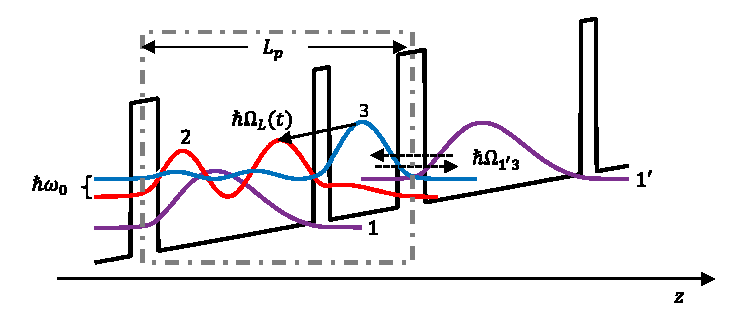
\includegraphics[width=9cm]{TOYMODEL.eps}\caption{Schematic
			diagram of a simple three-level LO-phonon depopulation THz QCL, where the
			upper laser level is populated via resonant tunneling.}%
		\label{fig:img01}%
	\end{figure}
	
	First, in order to illustrate the system of interest, let us take a simple
	toy model for a resonant phonon THz QCL, depicted in Fig. \ref{fig:img01}. In this
	configuration, we consider four relevant levels $\Ket{1'},\Ket{3},\Ket{2}$ and
	$\Ket{1}$ which are the injector level, the upper and lower laser levels and
	the depopulation level, which also serves as the injector level for the next
	period. The state $\Ket{1'}$ couples to $\Ket{3}$ via the anticrossing energy
	$\hslash\Omega_{1^{\prime}3}$, whereas the upper and lower laser levels interact
	via the instantaneous Rabi frequency $\Omega_{L}(t)=-ez_{32}E_{z}(t)/\hslash$.
	Here, $-ez_{32}=-e\Bra{3}\hat{z}\Ket{2}$ is the dipole matrix element,
	$E_{z}(t)$ is the electric field component along the growth direction $z$, and
	$e$ is the elementary charge. Lastly, we assume that the energy separation
	between $\Ket{1'}$ and $\Ket{3}$ is $\Delta_{1^{\prime}3}=\hslash\epsilon$ and
	that between the upper and lower laser levels $\Delta_{32}=\hslash\omega_{0}$.
	As it will be shown by our simulations, such a system possesses very rich and
	interesting dynamics, including effects such as anticrossing splitting, GVD,
	FWM, temporal and spatial hole burning and others.
	
	The electron transport can be treated quantum mechanically within the density
	matrix formalism, where the equation of motion (EOM) is given by the von
	Neumann equation
	\begin{equation}
		\frac{d\hat{\rho}}{dt}=\frac{\mathrm{i}}{\hslash}[\hat{\rho},\hat{H}].
		\label{eq:vonNeumann}%
	\end{equation}
	Here, $\hat{\rho}$ denotes the density operator, $\hat{H}$ the Hamiltonian of
	the system, and $[\cdot,\cdot]$ the quantum mechanical commutator. In general,
	$\hat{H}$ contains the various physical mechanisms that determine the overall
	carrier transport in the system. In view of the fact that we want to
	numerically solve Eq. (\ref{eq:vonNeumann}), we only include radiative
	transitions and resonant tunneling fully quantum mechanically, while we treat
	all incoherent scattering processes such as LO phonon, electron-electron,
	impurity and interface roughness scattering within a rate equation approach
	\cite{jirauschek2014modeling,iotti2005microscopic}.
	
	In THz QCLs, resonant tunneling plays an important role especially for thick
	barriers where the subbands involved in the electron transport have a small
	energy separation, which particularly applies to the injection barriers of
	various QCL\ designs
	\cite{callebaut2005importance,kumar2009coherence,dupont2010simplified}. This
	effect is usually treated in the so-called tight-binding (TB) approximation
	\cite{bastardwave}, where the wave functions are calculated for a single
	isolated period, and the electron subbands in adjacent modules are simply
	obtained by adequate translation in energy and space by the module length
	$L_{p}$ \cite{callebaut2005importance}. The energetic coupling between levels
	spanning the barrier between the modules is modelled by including the
	so-called anticrossing energies in the Hamiltonian matrix
	\cite{kumar2009coherence,dupont2010simplified}. In our case these are the
	injector and upper laser level, with the coupling energy $\hslash\Omega
	_{1^{\prime}3}$. In this tight-binding basis, the von Neumann equation reads
	\begin{align}
		&  \frac{d}{dt}%
		\begin{pmatrix}
			\rho_{1^{\prime}1^{\prime}} & \rho_{1^{\prime}3} & \rho_{1^{\prime}2}\\
			\rho_{31^{\prime}} & \rho_{33} & \rho_{32}\\
			\rho_{21^{\prime}} & \rho_{23} & \rho_{22}%
		\end{pmatrix}
		=\frac{\mathrm{i}}{\hslash}\left[
		\begin{pmatrix}
			\rho_{1^{\prime}1^{\prime}} & \rho_{1^{\prime}3} & \rho_{1^{\prime}2}\\
			\rho_{31^{\prime}} & \rho_{33} & \rho_{32}\\
			\rho_{21^{\prime}} & \rho_{23} & \rho_{22}%
		\end{pmatrix}
		,\overbrace{%
			\begin{pmatrix}
				\frac{\hslash\epsilon}{2} & \hslash\Omega_{1^{\prime}3} & 0\\
				\hslash\Omega_{1^{\prime}3} & -\frac{\hslash\epsilon}{2} & -\hslash\Omega_{L}(t)\\
				0 & -\hslash\Omega_{L}(t) & -\frac{\hslash\epsilon}{2}-\hslash\omega_{0}%
			\end{pmatrix}
		}^{\text{resonant tunneling and radiative coupling}}\right] \nonumber\\
		&  +\underbrace{%
			\begin{pmatrix}
				-\frac{\rho_{1^{\prime}1^{\prime}}}{\tau_{1^{\prime}}}+(\frac{1}%
				{\tau_{31^{\prime}}}+\frac{1}{\tau_{31}})\rho_{33}+(\frac{1}{\tau_{21^{\prime
						}}}+\frac{1}{\tau_{21}})\rho_{22} & \tau_{\parallel1^{\prime}3}^{-1}%
						\rho_{1^{\prime}3} & \tau_{\parallel1^{\prime}2}^{-1}\rho_{1^{\prime}2}\\
						\tau_{\parallel1^{\prime}3}^{-1}\rho_{31^{\prime}} & \frac{\rho_{1^{\prime
								}1^{\prime}}}{\tau_{1^{\prime}3}}-\frac{\rho_{33}}{\tau_{3}}+\frac{\rho_{22}%
						}{\tau_{23}} & \tau_{\parallel32}^{-1}\rho_{32}\\
						\tau_{\parallel1^{\prime}2}^{-1}\rho_{21^{\prime}} & \tau_{\parallel32}%
						^{-1}\rho_{32} & \frac{\rho_{1^{\prime}1^{\prime}}}{\tau_{1^{\prime}2}}%
						+\frac{\rho_{33}}{\tau_{32}}-\frac{\rho_{22}}{\tau_{2}}%
					\end{pmatrix}
				}_{\text{scattering rates matrix}}, \label{eq:vonNeumannmatrix}%
			\end{align}
			where $\rho_{ij}=\Bra{i}\hat{\rho}\Ket{j}$ are the corresponding density
			matrix elements and we have set the zero energy at $(E_{1^{\prime}}+E_{3})/2$.
			Furthermore $\tau_{ij}^{-1}$ denotes the outscattering rate from level $i$ to
			level $j$, $\tau_{i}$ is the lifetime of level $i$ with $\tau_{i}^{-1}%
			=\sum_{j\neq i}\tau_{ij}^{-1}$, and
			\[
			\tau_{\parallel ij}^{-1}=\frac{1}{2}\left(  \frac{1}{\tau_{i}}+\frac{1}%
			{\tau_{j}}\right)  +\frac{1}{\tau_{pure}}%
			\]
			is the damping rate of the coherence between levels $i$ and $j$, containing
			lifetime broadening and a ''pure'' dephasing rate $\tau_{pure}^{-1}$
			\cite{callebaut2005importance}.
			
			Notice that in Eq. (\ref{eq:vonNeumannmatrix}) we have omitted the time
			evolution related to state $\Ket{1}$, because it serves as the injector level
			for\ the next period, which allows us to eliminate it from the model by
			employing ''periodic'' boundary conditions in the scattering rates matrix. It
			is vital for the simulation that these periodic boundary conditions are
			implemented correctly, because our model is formulated in a manner which does
			not phenomenologically include the injection current density $J$ into the
			equations. Instead, we assume a periodic system where all carriers that reach
			the depopulation level $\Ket{1}$ are immediately re-injected into the system
			through level $\Ket{1'}$. In such a configuration the overall carrier density
			has to be conserved, which means that the relation $\sum_{j}d\rho_{jj}/dt=0$
			has to be satisfied at all times. Then, the current injected into the system
			is essentially equal to the current entering into the depopulation level,
			$\Ket{1}$. From rate equation analysis, the current density through such the
			system with volume-averaged carrier concentration $N$ is given by
			\cite{kumar2009coherence}
			\begin{equation}
				J=-eNL_{p}\left(  \sum_{j=2}^{3}\frac{\rho_{jj}}{\tau_{j1}}+\frac
				{\rho_{1^{\prime}1^{\prime}}}{\tau_{1^{\prime}1}}\right)  .
			\end{equation}
			
			The coupling of the microscopic density matrix equations to the macroscopic
			Maxwell's equations is usually done via the incorporation of the polarization
			term in Maxwell's equations as the expectation value of the quantum mechanical
			dipole moment operator,
			\begin{equation}
				P_{z}=-N\Gamma\Tr\{\hat{\rho}e\hat{z}\}=-N\Gamma(ez_{32}\rho_{32}+ez_{23}%
				\rho_{23})=-N\Gamma ez_{32}(\rho_{32}+\rho_{23}), \label{eq:fullpolarization}%
			\end{equation}
			where $\Gamma$ is the spatial overlap factor between the optical field and the
			active region. Assuming no free electric charges and also weak inhomogeneity,
			the optical field is governed by the wave equation
			\cite{boyd2003nonlinear,jirauschek2014modeling}
			\begin{equation}
				\left(  \partial_{x}^{2}-\frac{n_{0}^{2}}{c^{2}}\partial_{t}^{2}\right)
				E_{z}=\frac{1}{\epsilon_{0}c^{2}}\partial_{t}^{2}P_{z}, \label{eq:fullwave}%
			\end{equation}
			where $x$ denotes the propagation direction, $c$ is the speed of light in
			vacuum, $n_{0}$ denotes the refractive index of the material, and
			$\epsilon_{0}$ is the permittivity of free space. 
				
			\subsection{Maxwell-Bloch equations for a Fabry-Perot resonator}
			\label{sec:MBFP}
			Let us consider a Fabry-Perot resonator of a
			certain length $L$, and employ the rotating wave (RWA) and the slowly varying
			envelope approximations (SVEA) \cite{boyd2003nonlinear,gordon2008multimode}.
			The optical field inside the cavity can be written as a superposition of
			forward and backward propagating waves
			\begin{equation}
				E_{z}(x,t)=\frac{1}{2}\left\{  f_{+}(x,t)\exp\left [  \mathrm{i}(k_{c}%
				x-\omega_{c}t)\right ]  +f_{-}(x,t)\exp\left [ -\mathrm{i}(k_{c}x+\omega
				_{c}t)\right ]  +c.c\right\}  , \label{eq:e-ansatz}%
			\end{equation}
			where ''c.c.'' denotes the complex conjugate of the preceding expression, the
			$+$ and $-$ signs specify the forward/backward propagating waves' envelopes,
			respectively, and $\omega_{c}$ and $k_{c}$ are the field's carrier frequency
			and wave number, related by $k_{c}=n_{0}\omega_{c}/c$. Since the superposition
			of two counter-propagating waves forms a standing wave, this will lead to the
			formation of an inversion grating along the propagation direction $x$, a
			phenomenon also known as spatial hole burning. Thus for the diagonal elements
			of the density matrix we make the following ansatz
			\begin{equation}
				\rho_{ii}(x,t)=\rho_{ii}^{0}(x,t)+\rho_{ii}^{+}(x,t)\exp\left(  2\mathrm{i}%
				k_{c}x\right)  +\rho_{ii}^{-}(x,t)\exp\left(  -2\mathrm{i}k_{c}x\right)  ,
				\label{eq:ii-ansatz}%
			\end{equation}
			where $\rho_{ii}^{+}=(\rho_{ii}^{-})^{\ast}$ are the inversion grating's
			amplitudes \cite{wang2007coherent}. Lastly, we decompose the coherences of the
			density matrix as 
			\begin{subequations}
				\centering
				\label{eq:cohansatz}%
				\begin{align}
					\rho_{32}(x,t)  &  =\eta_{32}^{+}(x,t)\exp\left[  \mathrm{i}(k_{c}x-\omega
					_{c}t)\right]  +\eta_{32}^{-}(x,t)\exp\left[  -\mathrm{i}(k_{c}x+\omega
					_{c}t)\right]  ,\label{eq:32ansatz}\\
					\rho_{1^{\prime}2}(x,t)  &  =\eta_{1^{\prime}2}^{+}(x,t)\exp\left[
					\mathrm{i}(k_{c}x-\omega_{c}t)\right]  +\eta_{1^{\prime}2}^{-}(x,t)\exp\left[
					-\mathrm{i}(k_{c}x+\omega_{c}t)\right]  ,\label{eq:12ansatz}\\
					\rho_{1^{\prime}3}(x,t)  &  =\rho_{1^{\prime}3}^{0}(x,t)+\rho_{1^{\prime}%
						3}^{+}(x,t)\exp\left(  2\mathrm{i}k_{c}x\right)  +\rho_{1^{\prime}3}%
					^{-}(x,t)\exp\left(  -2\mathrm{i}k_{c}x\right)  . \label{eq:13ansatz}%
				\end{align}
			\end{subequations}
			Notice that Eqs. (\ref{eq:32ansatz}) and (\ref{eq:12ansatz}) follow the
			electric field ansatz since the corresponding transition energies are in close
			resonance with the optical field. In contrast, the ansatz Eq.
			(\ref{eq:13ansatz}) is chosen in analogy to Eq. (\ref{eq:ii-ansatz}) for the
			diagonal elements since the term $\rho_{1^{\prime}3}$ is expected to oscillate
			only slowly due to the small energetic spacing between subbands $1^{\prime}%
			$\ and $3$.
				
			Finally, plugging Eqs. (\ref{eq:e-ansatz}), (\ref{eq:ii-ansatz}) and
			(\ref{eq:cohansatz}) into Eqs. (\ref{eq:vonNeumannmatrix}),
			(\ref{eq:fullpolarization}) and (\ref{eq:fullwave}) and invoking the rotating
			wave and slowly varying amplitude approximations, we obtain our model in its
			final form:			
\begin{enumerate}
\item {Propagation equations}
\begin{equation}
\frac{n_{0}}{c}\partial_{t}f_{\pm}\pm\partial_{x}f_{\pm}=-\mathrm{i}%
\frac{N\Gamma ez_{32}k_{c}}{\epsilon_{0}n_{0}^{2}}\eta_{32}^{\pm}-l_{0}f_{\pm
}, \label{eq:rtwave}%
\end{equation}
\item { Population densities}%
\begin{subequations}
\label{eq:diagonaldm}%
\begin{align}
\frac{d\rho_{1^{\prime}1^{\prime}}^{0}}{dt} &= \mathrm{i}\Omega_{1^{\prime}%
3}\left(  \rho_{1^{\prime}3}^{0}-\rho_{31^{\prime}}^{0}\right)  +\left(
\frac{1}{\tau_{31^{\prime}}}+\frac{1}{\tau_{31}}\right)  \rho_{33}^{0}+\left(
\frac{1}{\tau_{21^{\prime}}}+\frac{1}{\tau_{21}}\right)  \rho_{22}^{0}%
-\frac{\rho_{1^{\prime}1^{\prime}}^{0}}{\tau_{1^{\prime}}},\label{eq:rho11-dm} \\
\frac{d\rho_{1^{\prime}1^{\prime}}^{+}}{dt} &= \mathrm{i}\Omega_{1^{\prime}%
3}\left(  \rho_{1^{\prime}3}^{+}-\rho_{31^{\prime}}^{+}\right)  +\left(
\frac{1}{\tau_{31^{\prime}}}+\frac{1}{\tau_{31}}\right)  \rho_{33}^{+}+\left(
\frac{1}{\tau_{21^{\prime}}}+\frac{1}{\tau_{21}}\right)  \rho_{22}^{+}-\left(
\frac{1}{\tau_{1^{\prime}}}+4k_{c}^{2}D\right)  \rho_{1^{\prime}1^{\prime}}^{+},\label{eq:rtpop1grating}\\
\frac{d\rho_{33}^{0}}{dt} &= \mathrm{i}\Omega_{1^{\prime}3}\left(
\rho_{31^{\prime}}^{0}-\rho_{1^{\prime}3}^{0}\right)  +\mathrm{i}\frac
{ez_{32}}{2\hslash}\left(  f_{-}^{\ast}\eta_{32}^{-}+f_{+}^{\ast}\eta_{32}%
^{+}-c.c.\right)  +\frac{1}{\tau_{1^{\prime}3}}\rho_{1^{\prime}1^{\prime}}%
^{0}+\frac{1}{\tau_{23}}\rho_{22}^{0}-\frac{\rho_{33}^{0}}{\tau_{3}},\\
\frac{d\rho_{33}^{+}}{dt} &=\mathrm{i}\Omega_{1^{\prime}3}\left(
\rho_{31^{\prime}}^{+}-\rho_{1^{\prime}3}^{+}\right)  +\mathrm{i}\frac
{ez_{32}}{2\hslash}\left[  f_{-}^{\ast}\eta_{32}^{+}-f_{+}(\eta_{32}^{-})^{\ast
}\right]  +\frac{\rho_{1^{\prime}1^{\prime}}^{+}}{\tau_{1^{\prime}3}}%
+\frac{\rho_{22}^{+}}{\tau_{23}}-\left(  \frac{1}{\tau_{3}}+4k_{c}%
^{2}D\right)  \rho_{33}^{+},\label{eq:rtpop3grating}\\
\frac{d\rho_{22}^{0}}{dt} &=-\mathrm{i}\frac{ez_{32}}{2\hslash}\left(
f_{-}^{\ast}\eta_{32}^{-}+f_{+}^{\ast}\eta_{32}^{+}-c.c.\right)  +\frac
{1}{\tau_{1^{\prime}2}}\rho_{1^{\prime}1^{\prime}}^{0}+\frac{1}{\tau_{32}}%
\rho_{33}^{0}-\frac{\rho_{22}^{0}}{\tau_{21}},\\
\frac{d\rho_{22}^{+}}{dt} &=-\mathrm{i}\frac{ez_{32}}{2\hslash}\left[
f_{-}^{\ast}\eta_{32}^{+}-f_{+}(\eta_{32}^{-})^{\ast}\right]  +\frac{1}%
{\tau_{1^{\prime}2}}\rho_{1^{\prime}1^{\prime}}^{+}+\frac{1}{\tau_{32}}%
\rho_{33}^{+}-\left(  \frac{1}{\tau_{2}}+4k_{c}^{2}D\right)  \rho_{22}^{+},
\label{eq:rtpop2grating}%
\end{align}
\end{subequations}
\item {Coherence terms}%
\begin{subequations}%
\label{eq:coherencesdm}
\begin{align}
\frac{d\rho_{1^{\prime}3}^{0}}{dt} &=-\mathrm{i}\epsilon\rho_{1^{\prime}%
3}^{0}+\mathrm{i}\Omega_{1^{\prime}3}\left(  \rho_{1^{\prime}1^{\prime}}%
^{0}-\rho_{33}^{0}\right)  +\mathrm{i}\frac{ez_{32}}{2\hslash}\left(
f_{+}^{\ast}\eta_{1^{\prime}2}^{+}+f_{-}^{\ast}\eta_{1^{\prime}2}^{-}\right)
-\tau_{\parallel1^{\prime}3}^{-1}\rho_{1^{\prime}3}^{0},\\
\frac{d\rho_{1^{\prime}3}^{\pm}}{dt}&=-\mathrm{i}\epsilon\rho_{1^{\prime}%
3}^{\pm}+\mathrm{i}\Omega_{1^{\prime}3}\left(  \rho_{1^{\prime}1^{\prime}%
}^{\pm}-\rho_{33}^{\pm}\right)  +\mathrm{i}\frac{ez_{32}}{2\hslash}f_{\mp}%
^{\ast}\eta_{1^{\prime}2}^{\pm}-\left(  \tau_{\parallel1^{\prime}3}%
^{-1}+4k_{c}^{2}D\right)  \rho_{1^{\prime}3}^{\pm},\label{eq:rho13grating}\\
\frac{d\eta_{32}^{\pm}}{dt} & =\mathrm{i}\left(  \omega_{c}-\omega_{0}\right)
\eta_{32}^{\pm}+\mathrm{i}\frac{ez_{32}}{2\hslash}\left[  f_{\pm}(\rho_{33}%
^{0}-\rho_{22}^{0})+f_{\mp}(\rho_{33}^{\pm}-\rho_{22}^{\pm})\right]
-\mathrm{i}\Omega_{1^{\prime}3}\eta_{1^{\prime}2}^{\pm}-\tau_{\parallel
32}^{-1}\eta_{32}^{\pm},\\
\frac{d\eta_{1^{\prime}2}^{\pm}}{dt} & =\mathrm{i}\left(  \omega_{c}%
-\omega_{0}-\epsilon\right)  \eta_{1^{\prime}2}^{\pm}+\mathrm{i}\frac{ez_{32}%
}{2\hslash}\left(  f_{\pm}\rho_{1^{\prime}3}^{0}+f_{\mp}\rho_{1^{\prime}3}^{\pm
}\right)  -\mathrm{i}\Omega_{1^{\prime}3}\eta_{32}^{\pm}-\tau_{\parallel
1^{\prime}2}^{-1}\eta_{1^{\prime}2}^{\pm}. \label{eq:rho12-dm}%
\end{align}
\end{subequations}
\end{enumerate}

	Notice that in Eq. (\ref{eq:rtwave}) we have phenomenologically added a linear
	amplitude loss coefficient $l_{0}$, and in Eqs. (\ref{eq:rtpop1grating}),
	(\ref{eq:rtpop3grating}), ({\ref{eq:rtpop2grating}), (\ref{eq:rho13grating}) a
		diffusion term $4k_{c}^{2}D$ describing the diffusion rate at which carriers
		diffuse away from peaks of the population grating. Here $D$ denotes the
		diffusion constant, which for GaAs/AlGaAs systems is }${46\,\mathrm{cm}^{2}%
		/}\mathrm{s}${ \cite{wang2009mode,vukovic2016multimode}. }
	The fields $f_{\pm }$ in Eq. (\ref{eq:rtwave}) satisfy the boundary conditions
	$f_{+}\left( 0\right) =rf_{-}\left( 0\right) $ and
	$rf_{+}\left( L\right) =f_{-}\left( L\right) $ \cite{wang2007coherent},
	where we set the reflection coefficient $r=1$ and instead include mirror outcoupling
	into the loss coefficient $l_{0}$. In Appendix
	\ref{sec:numerics}, the numerical methods used to solve Eqs. (\ref{eq:rtwave}%
	), (\ref{eq:diagonaldm}) and (\ref{eq:coherencesdm}) are briefly discussed.
	
	\section{Theoretical analysis of an LO phonon depopulation THz QCL with a strong injector anticrossing}
	\label{sec:application}
	In this section we extend our three level model, outlined in Sec. \ref{sec:thmodel}, to simulate one of the best performing QCL based THz frequency combs so far, the QCL design in
	\cite{burghoff2014terahertz}. This laser is based on a resonant LO phonon
	depopulation active region lasing at the central frequency $f_{0}%
	\approx3.5{\,}\mathrm{THz}$, and has been shown to produce a stable comb
	spectrum containing more than 70 equidistant longitudinal modes in a free
	running regime of operation. At optimum bias, field autocorrelation
	measurements indicate multimode lasing, and radio frequency (RF) measurements
	produce a very strong and narrow beatnote with a minimum reported full width
	at half-maximum (FWHM) linewidth of approximately $1.53{\,}\mathrm{kHz}$,
	indicating that at least part of the modes are phase-locked
	\cite{hugi2012mid,burghoff2014terahertz,wienold2014evidence,rosch2015octave}.
	Furthermore, a novel comb coherence detection technique, shifted-wave
	interference Fourier-transform (SWIFT) spectroscopy, has been developed to
	prove the stability of the THz comb over a large number of round trips
	\cite{burghoff2015evaluating}. To correctly describe the device under test, we
	first determine operating regimes where the ''single resonant tunneling and
	single optical transition'' assumption, made in Sec. \ref{sec:thmodel}, is justified.
	
	Fig. \ref{fig:img02}a illustrates the calculated wave functions at a bias of
	$11{\,}\mathrm{kV}/\mathrm{cm}$ obtained with the tight-binding approximation.
	From graphical inspection we see that there are in total five relevant
	levels per period, which we will refer to, according to their assumed role, as
	$\Ket{ULL}$ for the upper laser level, $\Ket{LLL1}$ for the higher energy
	level from a pair of lower laser levels, $\Ket{LLL2}$ for the lower energy
	level from the same pair, $\Ket{DEP1}$ for the higher energy level from a
	doublet of depopulation levels, and finally $\Ket{DEP2}$ for the lowest energy
	level. Furthermore, since the structure is periodic, the depopulation levels
	from the previous period will be referred to as $\Ket{INJ1}$ and $\Ket{INJ2}$, respectively.
	
	\begin{figure}[h!]
		\begin{center}
			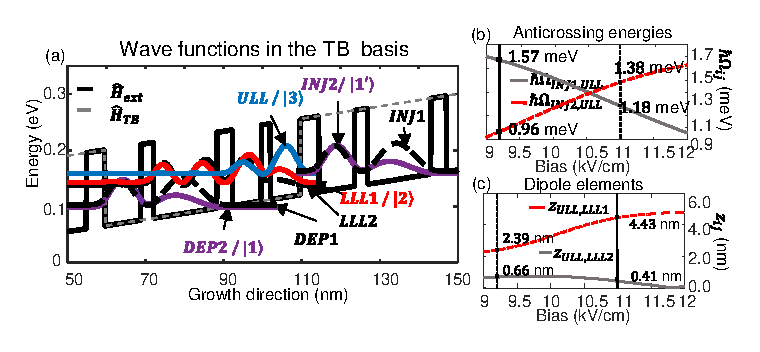
\includegraphics[width=10cm]{FL183S.eps}
		\end{center}
		\caption{\textbf{a}, The moduli squared of the wave functions of the THz QCL
			in \cite{burghoff2014terahertz} within the tight-binding approximation.
			\textbf{b}, The anticrossing coupling strengths between the pair of injector
			levels, $\ket{INJ1},\ket{INJ2}$, and the upper laser level $\ket{ULL}$,
			computed via the method outlined in \cite{bastardwave}. \textbf{c}, Dipole
			elements calculated for the same laser, obtained with the extended basis
			Hamiltonian, $\hat{H}_{ext}$.}%
		\label{fig:img02}%
	\end{figure}
	
	Figs. \ref{fig:img02}b and \ref{fig:img02}c depict the calculated coupling
	strengths $\hslash\Omega_{ij}$ between the injector states and the upper laser
	level for different biases, as well as the magnitudes of the dipole matrix
	elements, $\left| z_{ij}\right|  $, between the upper laser level and the
	doublet of lower laser levels. The anticrossing (AC) energies were calculated via
	the method described in \cite{bastardwave}, and the numerical values were
	verified by diagonalization of the tight-binding Hamiltonian. Focusing on bias
	values at around $11{\,}\mathrm{kV}/\mathrm{cm}$, our calculations show that
	there is almost perfect energetic alignment between $\Ket{INJ2}\ $and
	$\Ket{ULL}$, whereas $\Ket{INJ1}$ and $\Ket{ULL}$ are separated by
	approximately $\Delta_{INJ1,ULL}\approx4.3{\,}\mathrm{meV}$ (not shown in the
	figure). Even though the anticrossing energies $\hslash\Omega_{INJ1,ULL}%
	\approx1.18{\,}\mathrm{meV}$ and $\hslash\Omega_{INJ2,ULL}\approx1.38{\,}%
	\mathrm{meV}$ are of comparable strength, the strong resonance condition
	between the pair $\Ket{INJ2}$, $\Ket{ULL}$ enhances the tunneling probability,
	i.e. reduces the tunneling time, between those levels
	\cite{williams2007terahertz}, as compared to the tunneling transition between
	$\Ket{INJ1}$ and $\Ket{ULL}$. This means that the majority of the tunneling
	electrons will prefer the $\Ket{INJ2}\leftrightarrow\Ket{ULL}$ transport
	channel and hence our model, which includes only a single tunneling
	transition, ought to correctly capture the microscopic dynamics of the real
	device. From dipole moment calculations in Fig. \ref{fig:img02}c, we see that
	the optical transition at $11{\,}\mathrm{kV}/\mathrm{cm}$ is most likely to
	occur between the pair $\Ket{ULL}$, $\Ket{LLL1}$, and thus we can assign the
	state $\Ket{2}$ in our equations to be subband $\Ket{LLL1}$ from the system
	under investigation. Similarly, due to the discussion above, we can set the
	injector level in our reduced model, i.e. $\Ket{1'}$, to state $\Ket{INJ2}$.
	Finally, we can map $\Ket{3}$ to subband $\Ket{ULL}.$ The remaining states
	$\Ket{INJ1}$ and $\Ket{LLL2}$ are then treated within a rate equations
	approach and included into the scattering rates matrix by adequately extending
	Eq. (\ref{eq:vonNeumannmatrix}).
	
	\subsection{Gain and dispersion characterization}
	\label{subsec:numthztds} 
	In order to extract the spectral gain profile as well
	as the strength of the chromatic dispersion induced by the active region
	design, we have performed simulations emulating the THz time-domain
	spectroscopy (THz-TDS) technique, often used for gain characterization of THz
	QCLs \cite{burghoff2014broadband,jukam2008gain,martl2011gain}.
	
	We apply our model to a ring cavity configuration with length $L=2.5{\,}%
	\mathrm{mm}$ and neglect spatial hole burning effects which are not expected
	to play a role for this simulation. A weak unchirped Gaussian pulse is
	propagated inside the cavity for one round trip of length $L$. At each time step $t_{n}$ of our
	simulation, as well as at different points $x_{j}$ along the cavity length, we
	record the electric field envelope $f_{j}^{n}$ for further data processing.
	From this data the real and imaginary parts of the refractive index can be
	calculated in a straightforward manner, as briefly discussed below.
	
	In a ring cavity, we have only forward propagating waves (no standing waves)
	and thus the electric field can be written as
	\begin{equation}
		E(x,t)=\Re\{f(x,t)\exp\left[  \mathrm{i}(k_{c}x-\omega_{c}t)\right]
		\} ,
	\end{equation}
	where $f$ is the (slowly varying) envelope function. We will denote the
	electric field of the injected seed pulse at the input facet of our cavity as
	$E_{in}(t)$ and the field of the detected pulse as $E_{out}(t)$. Their Fourier
	transforms are $E_{in}(\omega)$ and $E_{out}(\omega)$, with the angular
	frequency $\omega$. The corresponding envelope functions are $f_{in}\left(
	t\right)  $ and $f_{out}\left(  t\right)  $, with the Fourier transforms
	$F_{in}\left(  \omega\right)  $ and $F_{out}\left(  \omega\right) $, respectively. For a
	weak seed pulse, the light-matter interaction is linear, and the active region
	can be described by its complex refractive index $\underline{n}\left(
	\omega\right)  =n^{\prime}\left(  \omega\right)  +\mathrm{i}n^{\prime\prime
	}\left(  \omega\right)  $, with the amplitude gain coefficient given by
	$g(\omega)=-n^{\prime\prime}(\omega)\omega/c$. The dependence between the seed
	and output field is then given by $E_{out}(\omega)=E_{in}(\omega)\exp\left(
	\mathrm{i}\omega\underline{n}L/c\right)  $, which corresponds to
	$F_{out}(\omega-\omega_{c})\exp(\mathrm{i}k_{c}L)=F_{in}(\omega-\omega
	_{c})\exp\left(  \mathrm{i}\omega\underline{n}L/c\right)  $. From this, we
	obtain
	\begin{align}
		n^{\prime}(\omega)  & =\frac{c}{L\omega}\angle\{F_{out}(\omega-\omega
		_{c})/F_{in}(\omega-\omega_{c})\}+\frac{ck_{c}}{\omega}, \\
		n^{\prime\prime}(\omega)  &  =-g(\omega)c/\omega=-\frac{c}{L\omega}%
		\log\{|F_{out}(\omega-\omega_{c})|/|F_{in}(\omega-\omega_{c})|\}.
		\label{eq:gaineq}%
	\end{align}
	
	Fig. \ref{fig:img03} shows the results from numerical THz-TDS simulations at a
	bias of $10.8{\,}\mathrm{kV/cm}$ for the active region in
	\cite{burghoff2014terahertz} for a single round trip of the seed THz
	pulse\textrm{.} All relevant simulation parameters, as well as the scattering
	times are given in Appendix \ref{sec:params}.
	
	\begin{figure}[h!]
		\begin{center}
			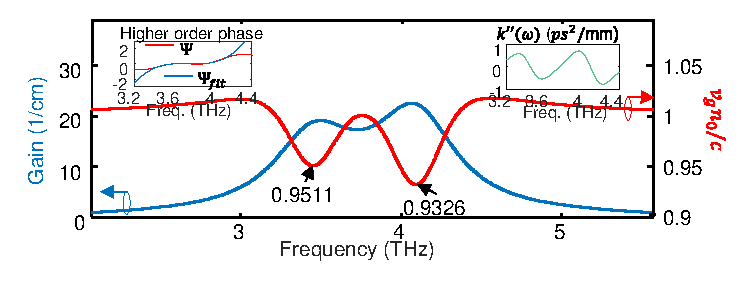
\includegraphics[width=10cm]{THZtds.eps}
		\end{center}
		\caption{Simulated spectral gain profile (blue curve, left y-axis) together
			with the normalized group velocity $v_{g}n_{0}/c$ (red curve, right y-axis).
			(Left inset) The higher order phase acquired by the test pulse upon propagating
			for 2.5 mm inside the laser cavity. (Right inset) The second derivative of the
			wave number with respect to the angular frequency (in units of ps$^{2}$/mm) as
			a measure af GVD. }%
		\label{fig:img03}%
	\end{figure}
	
	Since our aim was to probe the unsaturated gain profile, for these numerical
	experiments we used a weak seed pulse with a instantaneous Rabi frequency
	amplitude of $0.5{\,}\mathrm{ns}^{-1}$ and FWHM duration of $0.707{\,}%
	\mathrm{ps}$, corresponding to a FWHM bandwidth of $623{\,}\mathrm{GHz}$ for a
	transform limited pulse. In Fig. \ref{fig:img03} the blue curve illustrates
	the simulated spectral amplitude gain, obtained from Eq. (\ref{eq:gaineq}). We
	clearly can observe a pronounced splitting of the gain spectra into two
	frequency lobes, one centred around $3.55{\,}\mathrm{THz}$ and another one
	around $4.21{\,}\mathrm{THz}$. The red curve in Fig. \ref{fig:img03} depicts
	the frequency resolved group velocity, calculated from $v_{g}=[\partial
	k(\omega)/\partial\omega]^{-1}$ with $k(\omega)=n^{\prime}(\omega)\omega/c$,
	and normalized to the central frequency's phase velocity $c/n_{0}$.
	Due to the strong resonances at $3.55{\,}\mathrm{THz}$ and $4.21{\,}%
	\mathrm{THz}$, the low and high frequency components are delayed
	with respect to each other as $v_{g}n_{0}/c$ approaches $0.9511$ and $0.9326$
	for the low and high frequency gain peaks, respectively, where this ratio
	depends on the strength of the corresponding transition. The upper left inset
	of Fig. \ref{fig:img03} depicts the calculated higher order phase
	$\Psi=k(\omega)L$ (with the linear part removed) together with a third order
	polynomial fit to it, $\Psi_{fit}$, and shows that the dispersion relation
	within the spectral range of interest (i.e. from $3.5{\,}\mathrm{THz}$ to
	$4.2{\,}\mathrm{THz}$) is approximately cubic. Lastly, the top right inset
	illustrates the second derivative of the wave number with respect to
	frequency, i.e. $k''(\omega)$, which is a measure of GVD.
		
	From the above analysis we can conclude that even in the absence of bulk or
	waveguide dispersion, the doubly peaked resonant nature of the transition will
	cause significant dispersion in the cavity which is expected to deteriorate
	the comb performance. Here a question naturally arises: ''How does the
	presence of strong chromatic dispersion impact the mode proliferation
	process?'' If the multimode behaviour of free running QCLs is due to FWM, as
	suggested in \cite{friedli2013four,khurgin2014coherent}, then one would
	intuitively expect that such a high GVD will violate the phase matching
	condition and thus yield this nonlinear process ineffective. However, from
	experiment \cite{burghoff2014terahertz,rosch2015octave}, multimode operation
	of both mid-infrared and THz QCLs could be observed, even in the presence of
	strong dispersion. To investigate further this question, we analyze the
	nature of this mode generation mechanism and estimate the amount of phase
	mismatch induced by the resonant transition.
	
	\subsection{Four wave mixing}
	\label{subsec:FWM}
	We have conducted numerical experiments, similar to the THz-TDs technique,
	where we pumped the 2.5 mm ring cavity laser, outlined above, with two frequencies
	$\omega_{1}$ and $\omega_{2}<\omega_{1}$. For 50 round trips we collected the
	signal and calculated the resulting power spectrum.
	
	\begin{figure}[h!]
		\begin{center}
			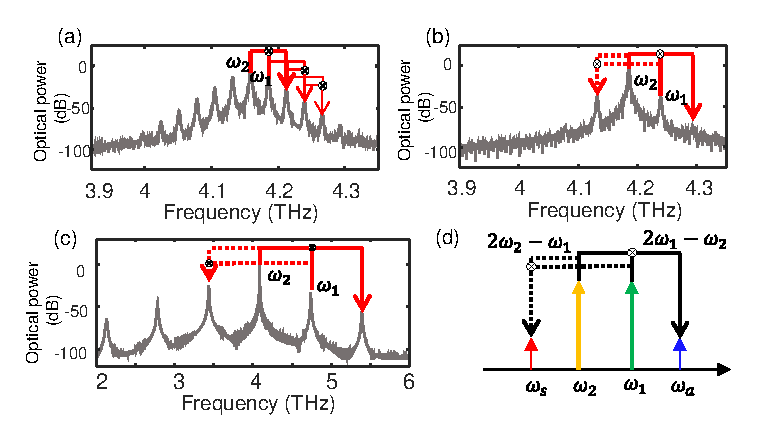
\includegraphics[width=10cm]{FWM.eps}
		\end{center}
		\caption{\textbf{a}, Optical spectrum
			obtained from THz-TDs simulations when the seed frequencies, $\omega_{1}$ and
			$\omega_{2}$, are separated by the free spectral range $\Delta\omega$.
			\textbf{b}, Same as \textbf{a}, however this time $\omega_{1}-\omega
			_{2}=2\Delta\omega$. \textbf{c}, Optical spectrum from simulations where the
			seed frequencies are distributed under both peaks of the spectral gain.
			\textbf{d}, Schematic representation of degenerate FWM
			\cite{butcher1991elements}, where two pump modes $\omega_{1}$,$\omega_{2}$
			combine to produce sidebands at frequencies $\omega_{a}=2\omega_{1}-\omega
			_{2}$ and $\omega_{s}=2\omega_{2}-\omega_{1}$.}%
		\label{fig:img04}%
	\end{figure}
	
	Figures \ref{fig:img04}a, b and c illustrate the results from these simulations when the seed frequencies
	$\omega_{1}$ and $\omega_{2}$ were varied. In Fig. \ref{fig:img04}a, we chose
	$\omega_{1}$ and $\omega_{2}$ to be separated by the free spectral range,
	$\Delta\omega=2\pi c/\left(  n_{0}L\right)  $, and to reside within the high
	frequency lobe of the spectrum. We can clearly observe the formation of
	side-modes separated by $\Delta\omega$, populating this whole frequency lobe.
	Similarly in Fig. \ref{fig:img04}b, our seed frequencies were chosen to be
	separated by $2\Delta\omega$ and again side-modes can be seen in the spectrum,
	however this time with mode spacing of $2\Delta\omega$. This kind of behaviour
	is a trademark of degenerate FWM described by susceptibilities $\chi
	(-\omega_{a};\omega_{1},-\omega_{2},\omega_{1})$ and $\chi(-\omega_{s}%
	;\omega_{2},-\omega_{1},\omega_{2})$ \cite{butcher1991elements}, where the
	pump modes $\omega_{1}$ and $\omega_{2}$ mix to produce a signal at the
	anti-Stokes and Stokes frequencies $\omega_{a}$ and $\omega_{s}$,
	respectively. This process is schematically illustrated in Fig.
	\ref{fig:img04}d. In Fig. \ref{fig:img04}a, b, $\omega_{1,2}$ are distributed
	around $4.2{\,}\mathrm{THz}$, and there is no activation of modes under the
	low-frequency lobe part of the spectrum. Such dynamics differs from simulations 
	at the same bias, but within a Fabry-Perot cavity, where we observe lasing 
	from both lobes of the gain, as will be discussed in the next section. 
	This means that in order for the FWM process to start, some kind of
	seeding mechanism is necessary. Since in these experiments we considered a
	ring-cavity laser, multimode instabilities such as spatial hole burning
	\cite{gordon2008multimode} were not included, and lasing only started in the
	lobe excited by the seed.\textrm{ }Lastly, Fig. \ref{fig:img04}c shows
	simulation results when both pump modes are chosen to be in resonance with the
	corresponding gain peaks, and again we observe the familiar formation of side
	modes due to FWM.
	
	The phase mismatch for the anti-Stokes component of the degenerate FWM
	process, depicted in Fig.\ref{fig:img04}a, is \cite{butcher1991elements}
	\begin{equation}
		L\Delta k=\left[  2k(\omega_{1})-k(\omega_{2})-k(\omega_{a})\right]  L,
	\end{equation}
	and similar for the Stokes component. For a Fabry-Perot laser of length $L$,
	we have $\Delta\omega=\pi c/\left(  n_{0}L\right)  $, and Taylor-expanding
	around $\omega_{1}$ up to third order in $\Delta\omega$ yields, with
	$\omega_{2}=\omega_{1}-\Delta\omega$ and $\omega_{a}=2\omega_{1}-\omega
	_{2}=\omega_{1}+\Delta\omega$,
	\begin{equation}
		L\Delta k=-L\Delta\omega^{2}\left.  \frac{\partial^{2}k}{\partial\omega^{2}%
		}\right|  _{\omega_{1}}+O(\Delta\omega^{4})\approx-\frac{1}{L}\left(
		\frac{\pi c}{n_{0}}\right)  ^{2}\left.  \frac{\partial^{2}k}{\partial
			\omega^{2}}\right|  _{\omega_{1}}.\label{eq:phasemismatch}
	\end{equation}
	Plugging in typical values of $L=5$ mm, $n_{0}=3.6$ and $\partial_{\omega}%
	^{2}k\approx2{\,}\mathrm{ps}^{2}/\mathrm{mm}$ as an upper estimate for GVD, we
	obtain a phase mismatch of $L\left|  \Delta k\right|  =0.0274{\,}\mathrm{rad}%
	$, which is negligible. In fact, from Eq. (\ref{eq:phasemismatch}) it can be deduced that the 
	phase matching condition is further enhanced by the length $L$ of the cavity. This means that despite significant dispersion present
	in the cavity, under the favourable conditions of broadband gain, strong third
	order nonlinearity and some kind of multimode instability mechanism, such
	lasers can potentially emit a multitude of longitudinal modes even in a free
	running regime of operation, as reported in numerous experiments
	\cite{wienold2014evidence,burghoff2014terahertz,hugi2012mid,rosch2015octave}.
	
	\section{Simulation of comb operation and comparison to experiment}
	\label{sec:tdsims}
	In this section, we present simulation results for comb operation of the
	device in \cite{burghoff2014terahertz}, now considering counterpropagating
	waves in the Fabry-Perot cavity with a length $L=5{\,}\mathrm{mm}$, giving
	rise to spatial hole burning. Our simulations only use the device
	specifications and well known material parameters as an input, with the
	exception of empirical dephasing times. Again, the electron wavefunctions and
	eigenenergies are computed with a Schr{\"{o}}dinger-Poisson solver, and the
	carrier lifetimes are extracted from Monte Carlo carrier transport
	simulations. The used model parameters are listed in Appendix \ref{sec:params}%
	. We propagate over $\sim$15000 round trips to obtain results close to steady state.
	
	\subsection{Frequency domain}
	In Fig. \ref{fig:img05}, we compare the calculated spectra and beatnotes from
	simulations without dispersion compensation (Fig. \ref{fig:img05}c,d) and with
	dispersion compensation (Fig. \ref{fig:img05}e,f) to experimental data (Fig.
	\ref{fig:img05}a,b). Here, the simulation bias is set slightly below
	resonance, i.e., at $10.8{\,}\mathrm{kV}/\mathrm{cm}$. In both the dispersion
	compensated and uncompensated case, we observe reasonable agreement
	with the experimental optical power spectra (Fig. \ref{fig:img05}a), however
	substantial differences arise when we consider the corresponding
	beatnotes.

	
	Let us first discuss the simulation results in Fig. \ref{fig:img05}c, d. While
	experimental data show a strong and narrow beatnote with an FWHM linewidth of
	approximately $0.55{\,}\mathrm{MHz}$ (Fig. \ref{fig:img05}b), in Fig.
	\ref{fig:img05}d we observe a multi-beatnote signal distributed around
	$8.14{\,}\mathrm{GHz}$. This deviates from the experimental value of
	around\textrm{ }$6.8${\thinspace}$\mathrm{GHz}$ because the experimental
	implementation of GVD compensation in the cavity results in an increased
	effective cavity length. In the RF spectrum of Fig \ref{fig:img05}d, we can
	distinguish two peaks, one at $8.149{\,}\mathrm{GHz}$ and another at
	$8.151{\,}\mathrm{GHz}$, both with an FWHM of approximately $3{\,}%
	\mathrm{MHz}$ (Fourier transformation of 10$^{4}$ round trips yields a
	frequency resolution of $0.83{\,}\mathrm{MHz}$, where at least two frequency
	intervals are required to resolve the peak). From the group velocity delay
	plot in Fig. \ref{fig:img03} as well as from the spectra in Fig.
	\ref{fig:img05}c we can deduce that since the high frequency lobe's spectral
	components carry more power and have lower group velocity $v_{g}$, the
	stronger peak in the beatnote belongs to those frequency components, whereas
	the weaker one is associated with the lower frequency modes. This means that
	there ought to be two co-propagating pulses, albeit with a different $v_{g}$,
	which interfere in the beatnote measurement to produce the chaotic RF spectrum
	in Fig. \ref{fig:img05}d. The amount of noise in this non-comb regime of
	operation can be therefore traced mainly to the timing jitter induced by the
	difference in group velocities of those pulses. This will be elaborated
	further below, when we consider our results in the time domain.
	
	\begin{figure}[h!]
			\begin{center}
				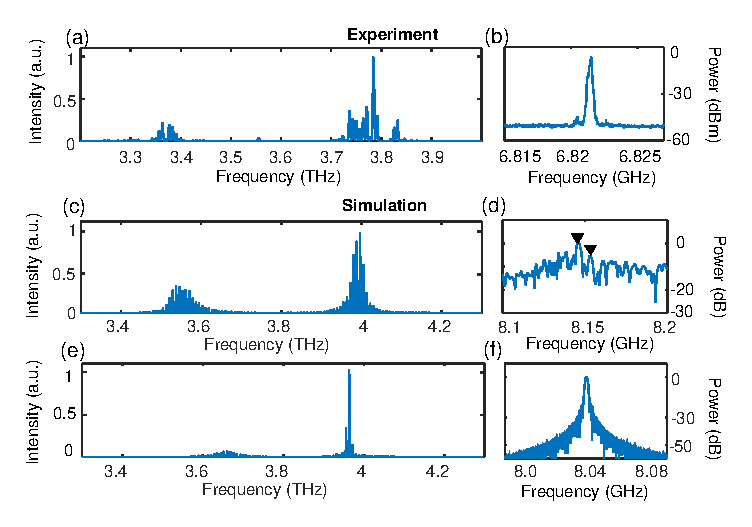
\includegraphics[width=8cm]{SPECTRA_EXPERIMENT.eps}
			\end{center}
			\caption{ Optical power spectra (left column) and beatnotes (right column)
				from experiment and simulations of the device in \cite{burghoff2014terahertz}.
				\textbf{a},\textbf{b} Experimental data for the dispersion compensated laser,
				at driving current of $0.9$ A. Simulation results without dispersion
				compensation (\textbf{c} and \textbf{d}) and with dispersion compensation
				(\textbf{e} and \textbf{f}). The experimentally detected beatnote in
				\textbf{b} has a FWHM of approx. 0.553MHz, whereas the simulated beatnote in
				\textbf{f} has a resolution limited FWHM of 1.66MHz. The strongest peak in \textbf{d}
				has a FWHM of 3.04 MHz.}%
			\label{fig:img05}%
		\end{figure}
		
	The situation drastically changes when we employ dispersion compensation in
	our simulations. To cancel the accumulated higher order phase components,
	after each round trip we Fourier-transform the electric field envelope,
	subtract from the resulting phasor the phase $\Psi$, extracted analogously to the simulation
	in Fig. \ref{fig:img03}, and inverse Fourier-transform the result. The
	obtained spectral power density and RF spectra are plotted in Fig.
	\ref{fig:img05}e,f. We see that such a procedure equilibrates the difference
	in the group velocities of different lasing modes, which results in a single, strong and narrow beatnote with a linewidth corresponding to our numerical frequency resolution, as expected from the experimental results for comb operation in Fig. \ref{fig:img05}b.
	
	\subsection{Time domain}
	\label{sec:timedomain}	
	In \cite{burghoff2015evaluating} it was shown that the strong injector
	anticrossing leads to a splitting of the emitted comb spectra in frequency
	domain and to an effect which was coined as ''temporal hole burning'' in time
	domain. To compare our simulation results to experiment, we applied a low-pass
	and high-pass finite impulse response filter to the simulated electric field,
	in order to separate the low and high frequency lobe components of the signal,
	respectively. Since the experimental design is dispersion compensated, we
	first consider this case in our simulation, corresponding to the results in
	Fig. \ref{fig:img05}e, f. The smoothed experimental and simulated
	instantaneous intensity are depicted in Fig. \ref{fig:img06}a and b,
	respectively, with a smoothing length of\textrm{ }$10{\,}\mathrm{ps}$ in experiment
	and $3{\,}\mathrm{ps}$ in simulation.
		
	\begin{figure}[h!]
		\begin{center}
			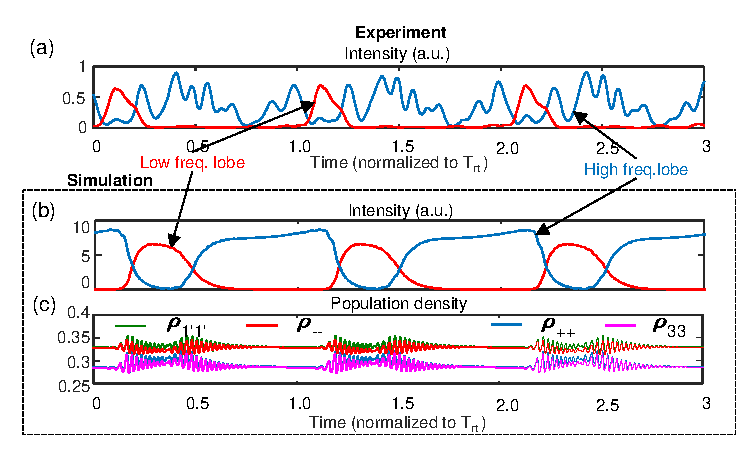
\includegraphics[width=9cm]{TEMPHOLEBURNING_EXPERIMENT.eps}
		\end{center}
		\caption{Time domain separation of the optical field into high and low
			frequency lobe components. \textbf{a} Measured intensity over time from
			\cite{burghoff2015evaluating} for the same THz comb device as in
			\cite{burghoff2014terahertz}, driven with $0.9{\,}\mathrm{A}$ current.
			\textbf{b} Simulated intensity over time for a dispersion compensated QCL
			evolved for $\sim$15000 round trips. \textbf{c} Time dependent populations the
			injector and upper laser level ( i.e. $\rho_{1'1'}$, $\rho_{33}$) as well as the dressed states (i.e. $\rho_{++}$, $\rho_{--}$).}%
		\label{fig:img06}%
	\end{figure}
		
	We note that when the population dynamics is extremely fast,
	memory effects become relevant, which can be taken into account by using a non-Markovian approach \cite{butscher2005ultrafast, knezevic2013time}, however at the cost of
	considerably increased numerical complexity. Since the modeling of frequency comb
	operation requires simulations over many 1000 round trips as discussed above,
	we rely on our model Eqs. (\ref{eq:rtwave})--(\ref{eq:coherencesdm})
	where the scattering transitions are implemented by corresponding rates.
	This approach already yields decent agreement between experiment and simulation as both data
	demonstrate a pulse switching behaviour between the high and low frequency
	lobe components of the spectra. The high frequency lobe pulse (blue curve) has
	a longer time duration than the low lobe signal (red curve). We believe this
	results from the difference in relative strengths of the corresponding
	spectral lobes, as the high lobe components experience more gain (Fig.
	\ref{fig:img03}). Furthermore, in the experimental trace an additional
	oscillatory substructure emerges, the reason for which remains to be clarified. However, a possible explanation could be 
	the presence of windowing effects of the Fourier transform spectrometer. 

	
	The dependence of the relative strengths of both lobes on the bias\textrm{
	}has already been discussed in \cite{dupont2010simplified}, however its
	implications on the time domain behaviour of the laser were not considered in
	greater detail. To summarize the conclusions in \cite{dupont2010simplified},
	the inclusion of a strong injector anticrossing leads to a splitting of the
	injector $\Ket{1'}$ and upper laser level $\Ket{3}$ into a doublet of
	so-called ''dressed states''. The higher energy level is denoted by $\Ket{+}$
	(also known as the ''anti-symmetric'' state), and the other level by $\Ket{-}$
	(i.e. the ''symmetric'' state). These states are separated by approximately
	the anticrossing energy $2\hslash\Omega_{1^{\prime}3}$ (depending on the
	detuning), which can be readily confirmed from experiment
	\cite{burghoff2014terahertz}. The relative radiative coupling strength of
	states $\Ket{+}$ and $\Ket{-}$ with the lower laser level depends on the
	detuning from resonance. Assuming low intracavity intensity, it can be shown
	that below the resonant bias, i.e., for $\hslash\epsilon<0$, the high frequency
	lobe of the gain dominates the transition, whereas above resonance the low
	lobe does (see Appendix \ref{sec:biasdependence}). As our simulations and
	experimental data show, this results in a longer high frequency pulse.
	
	Fig. \ref{fig:img06}c displays the calculated density matrix elements
	$\rho_{33}$, $\rho_{++}$, $\rho_{--}$ and $\rho_{1'1'}$ as a function of time. 
	For all four terms, we observe dampened Rabi-oscillations upon a pulse switching event, 
	which manifests the coherent population dynamics due to resonant tunneling. The
	period of these oscillations is approximately $2.84{\,}\mathrm{ps}$, giving us a frequency of $350{\,}\mathrm{GHz}$,
	which is namely the beat frequency between the high and low lobes of the dispersion compensated laser's spectrum
	(see Fig. \ref{fig:img05}). We can also clearly observe that whenever the high
	frequency lobe lases, state $\Ket{+}$ gets more strongly depleted, whereas 
	whenever the low lobe is switched on, state $\Ket{-}$ saturates. 
	
	\begin{figure}[h!]
		\begin{center}
			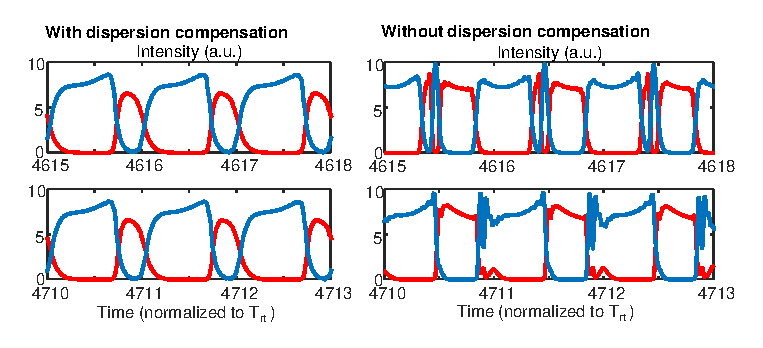
\includegraphics[width=10cm]{TEMPHOLEBURNING.eps}
		\end{center}
		\caption{Simulated high (blue) and low (red) frequency pulses for a
			numerically dispersion compensated (left column) and an uncompensated (right
			column) THz QCL. Data from round trip 4615-4618 (top) and
			4710-4713 (bottom) are shown.}%
		\label{fig:img07}%
	\end{figure}
	
	Lastly, to illustrate the implications of the existence of co-propagating high
	and low frequency lobe pulses in the presence of GVD, the simulated
	instantaneous intensities with (left column) and without (right column)
	dispersion compensation are shown in Fig. \ref{fig:img07} for different
	temporal intervals. Temporal hole burning, or pulse switching, is clearly
	present in both cases. For dispersion compensation, the periodicity is
	preserved over many round trips, as can be seen by comparing the intensity
	traces for the two displayed temporal intervals. By contrast, in the presence
	of GVD the high and low frequency lobes constantly compete with each other,
	which leads to a complex non-periodic temporal shape of the signal. Thus, while
	the signal from a low GVD QCL has a minimal timing jitter, which results in a
	narrow and strong beatnote, the one from a dispersion uncompensated device
	operates in a multi-pulse regime with a complicated temporal and spectral
	profile, and thus never quite reaches a steady state.
	
	One can naturally extrapolate these conclusions to a situation where the
	effects of material and waveguide dispersion add to a much more complicated
	dispersion profile, as compared to the one in Fig. \ref{fig:img03}. In such a
	case, the competition between electric field signals propagating with various
	different group velocities will lead to a chaotic and unstable beatnote,
	characteristic for multimode non-comb behaviour of QCLs, often observed in
	experiment \cite{burghoff2014terahertz,wienold2014evidence,rosch2015octave}.
	
	\section{Conclusion}
	We have presented a theoretical model suitable for the simulation of THz QCLs
	in comb and non-comb regimes of operation, based on the full numerical
	solution of the Maxwell-Bloch equations in rotating wave approximation. We
	have shown that our approach correctly captures the complicated dynamics
	between four wave mixing, coherent tunneling and spectral gain splitting,
	group velocity dispersion, as well as spatial hole burning, as it delivers
	simulation results in good agreement with experimental data. We have used this
	model to characterize the spectral gain profile and the corresponding group
	velocity delay, and to investigate the FWM as the dominant comb proliferation
	mechanism. Simulations of comb operation yielded a spectral comb shape in good
	agreement with experiment, and the the temporal switching behaviour between
	the high and low frequency components reported in experiment could also be
	reproduced. Furthermore, we have demonstrated that in contrast to earlier theoretical approaches our model can also capture non-ideal comb operation and transitions between comb and
	non-comb operating regimes.
	
	\section*{Acknowledgments}
	This work was supported by the German Research Foundation (DFG) within the
	Heisenberg program (JI 115/4-1) and under DFG Grant No. JI 115/9-1.

\begin{appendices}%
\section{Numerics}
\label{sec:numerics}
Eqs. (\ref{eq:rtwave}), (\ref{eq:diagonaldm}) and
(\ref{eq:coherencesdm}) comprise a system of two partial and thirteen ordinary
differential equations. As there is no known analytical solution for this
system, we time step the latter numerically with the aid of carefully chosen
schemes. The field propagation equations, Eq. (\ref{eq:rtwave}), are a pair of
inhomogeneous hyperbolic equations the accurate numerical solution of which is
far from trivial. From the area of computational fluid dynamics
\cite{wesseling2009principles}, it is known that a simple central differences
discretization scheme for Eq. (\ref{eq:rtwave}) will be highly unstable due to
the introduction of strong \emph{numerical} dispersion near sharp edges or
discontinuities of the solution. A finite difference scheme that does not
generate such spurious oscillations is called monotonicity preserving
\cite{wesseling2009principles} and its usage is essential for the correct
interpretation of simulation results, especially when one tries to quantify
the amount of \emph{physical} dispersion present. Without getting too much
into detail, we present a second order linear finite difference discretization
scheme, possessing the monotonicity preserving property (in the case when
$\eta_{\pm}\propto f_{\pm}$), for the model equation
\begin{equation}
	\frac{\partial f_{\pm}}{\partial t}=\mp c\frac{\partial f_{\pm}}{\partial
		x}+\eta_{\pm}(x,t)+kf_{\pm}.\label{eq:genericwave}%
\end{equation}
We take an equidistant spatio-temporal grid with grid size $\Delta x$ and time
step $\Delta t$ and set the values of the grid variables at spatial point
$x_{m}=m\Delta x$ and time $t_{n}=n\Delta t$ as $f_{\pm}(m,n)$, where the
$\pm$ index denotes the forward/backward propagating envelopes, respectively, and $\eta_{\pm}$ denotes the corresponding source terms. The time stepping scheme we use is based on a second order upwind
discretization, first introduced by Risken and Nummedal \cite{risken1968self},
and is given by
\begin{align}
	f_{\pm}(m,n+1) &  =f_{\pm}(m\mp1,n)+\Delta t\left[  \eta_{\pm}(m,n)+kf_{\pm
	}(m,n)\right]  \nonumber\label{eq:riskennummedal}\\
	&  +\frac{\Delta t^{2}}{2}\left\{  \left[  \frac{\partial \eta_{\pm}}{\partial
		t}\right]  _{m}^{n}\mp c\left[  \frac{\partial \eta_{\pm}}{\partial x}\right]
	_{m}^{n}\mp2kc\left[  \frac{\partial f_{\pm}}{\partial x}\right]  _{m}%
	^{n}+k\eta_{\pm}(m,n)+k^{2}f_{\pm}(m,n)\right\}  ,
\end{align}
where the time step is chosen as $\Delta t=\Delta xn_{0}/c$, with $c/n_{0}$
being the velocity of light in the medium. The evaluation of the time
derivative of $\eta_{\pm}(x,t)$ can be computed analytically from the density matrix
equations, Eq. (\ref{eq:coherencesdm}). The terms in rectangular brackets, $\left[
\partial \eta_{\pm}/\partial x\right]  _{m}^{n}$ and $\left[  \partial f_{\pm
}/\partial x\right]  _{m}^{n}$, can be computed via forward/backward
finite differences, depending on the propagation direction of the field. 

The density matrix equations, Eqs. (\ref{eq:diagonaldm}) and
(\ref{eq:coherencesdm}), form a system of ordinary differential equations
and the usage of any out of the box numerical solver ought to suffice. In our
experience a suitable method which is high-order accurate and also preserves
the normalization property of the density matrix, i.e. $\Tr(\rho)=1$, is given
by the fifth order linear multi-step Adams-Bashforth method, calculating the
update of the time dependent variable as a linear combination of several past
time-steps
\begin{equation}
	y^{n+1}=y^{n}+\Delta t\sum\limits_{m=0}^{k-1}c_{m}F(y_{n-m},t_{n-m})\text{
	},\label{eq:adams-bashforth}%
\end{equation}
where again we have assumed the model equation
\begin{equation}
	\dot{y}(t)=F(y,t)\label{eq:adams-bashforth-model}%
\end{equation}
and $c_{n}$ are suitably chosen coefficients.

\section{Dependence of the dominant transition on bias}
\label{sec:biasdependence}
As we have already shown in Sec. \ref{subsec:numthztds}, the introduction of
the coupling energy $\hslash\Omega_{1^{\prime}3}$ into the Hamiltonian of the
system contributes to a splitting of the optical spectra into a high and a low
frequency lobe. This is due to the fact that the extended system's Hamiltonian
is non-diagonal in the tight binding basis. The new eigenstates, which
diagonalize the Hamiltonian in Eq. (\ref{eq:vonNeumannmatrix}), are the
so-called dressed states \cite{callebaut2005importance,dupont2010simplified},
which are obtained from $\Ket{1'}$ and $\Ket{3}$ via the unitary
transformation
\begin{align}
	\Ket{+} &  =\cos\theta\Ket{1'}-\sin\theta\Ket{3}%
	,\nonumber\label{eq:dressedstates}\\
	\Ket{-} &  =\sin\theta\Ket{1'}+\cos\theta\Ket{3}.
\end{align}
The corresponding energies are given by $E_{\pm}=\pm\hslash(\epsilon
^{2}+4\Omega_{1^{\prime}3}^{2})^{1/2}$, where the coefficients are computed from
$\tan\theta=-2\Omega_{1^{\prime}3}/[\epsilon+\left(  \epsilon^{2}%
+4\Omega_{1^{\prime}3}^{2}\right)  ^{1/2}].$ Here we remind the reader that we
have set the zero energy at $(E_{1^{\prime}}+E_{3})/2$ and that the detuning
from the $\Ket{1^{\prime}}\leftrightarrow\Ket{3}$ resonance is given by
$E_{1^{\prime}}-E_{3}=\hslash\epsilon$. Following \cite{dupont2010simplified},
the ratio of the dipole matrix elements for the $\Ket{+}\leftrightarrow\Ket
{2}$ and $\Ket{-}\leftrightarrow\Ket{2}$ transitions, which determines the
relative strength between the high and low frequency gain lobes, is
\[
\left|  \frac{\Bra{+}\hat{z}\Ket{2}}{\Bra{-}\hat{z}\Ket{2}}\right|
\approx|\tan\theta|=\frac{2|\Omega_{1^{\prime}3}|}{|\epsilon+\sqrt
	{\epsilon^{2}+4\Omega_{1^{\prime}3}^{2}}|},
\]
where we assume that $z_{1^{\prime}2}\approx0$. We now can easily see that at
high biases, i.e. positive detunings $\epsilon>0$, $|\tan\theta|<1$ and thus
the low frequency transition will have higher probability. On the other hand,
$|\tan\theta|>1$ for $\epsilon<0$ which will lead to lasing predominantly in
the high frequency regime.

\section{Simulation parameters}		
\label{sec:params}

In Table \ref{tab:table01} we summarize the parameter set
used for our simulations and in Table \ref{tab:table02}, the scattering rates
between each pair of the active region subbands calculated with our ensemble
Monte Carlo simulation code \cite{jirauschek2014modeling} is shown. The code
includes all relevant scattering mechanisms reported to play a role in quantum
cascade lasers, including longitudinal optical phonons, acoustic phonons,
interface roughness and impurity scattering as well as electron-electron
scattering. The calculated rates include all these mechanisms and are
presented in units of ps$^{-1}$.

\begin{table}[h!]
	\centering{\footnotesize
		\begin{tabular}
			[c]{p{35mm}cc}\hline
			\textbf{Parameter} & \textbf{Symbol} & \textbf{Value}\\\hline
			Avg. carrier density & N & 5.6$\times10^{15}\,$cm$^{-3}$\\
			Overlap factor & $\Gamma$ & 0.9\\
			Linear amplitude loss coeff. & $l_{0}$ & $11\,$cm$^{-1}$\\
			Dipole matrix element & $ez_{32}$ & 4.0 nm $\times e$\\
			Refractive index & $n_{0}$ & 3.6\\
			Diffusion constant & D & 46$\,$cm$^{2}$/s\\
			Left/right mirror reflectivity & $R_{L/R}$ & 0.8\\
			1'$\rightarrow$3 pure deph. time & $\tau_{1^{\prime}3}^{pure}$ & 0.6$\,$ps\\
			3 $\rightarrow$2 pure deph. time & $\tau_{32}^{pure}$ & 1$\,$ps\\
			1'$\rightarrow$2 pure deph. time & $\tau_{1^{\prime}2}^{pure}$ & 1$\,$ps\\
			3 $\leftrightarrow$ 2 resonance energy & $\Delta_{32}$ & 15.82$\,$meV\\
			1'$\leftrightarrow$ 3 detuning energy & $\Delta_{1^{\prime}3}$ &
			-0.43$\,$meV\\
			1'$\leftrightarrow$ 3 anticrossing energy & $\hslash\Omega_{1^{\prime}3}$ &
			-1.3447$\,$meV\\\hline
		\end{tabular}
	}\caption[Table caption text]{Simulation parameters for a THz QCL, modelled
	after the device in \cite{burghoff2014terahertz}. The model overlap factor and
	the facet reflectivities are selected based on \cite{kohen2005electromagnetic}
	for a metal-metal waveguide with thickness $10{\,}\mu\mathrm{m}$ and width of
	$20{\,}\mu\mathrm{m}$.}%
\label{tab:table01}%
\end{table}

\begin{table}[h]
\centering{\footnotesize
	\begin{tabular}
		[c]{r|ccccccc}\hline
		& \textbf{INJ1} & \textbf{INJ2} & \textbf{ULL} & \textbf{LLL1} & \textbf{LLL2}
		& \textbf{DEP1} & \textbf{DEP2}\\\hline
		\textbf{INJ1} & 0 & 0.8179 & 0.0200 & 0.0016 & 0.0007 & 0.0025 & 0.0029\\
		\textbf{INJ2} & 0.4906 & 0 & 0.0451 & 0.0016 & 0.0007 & 0.0024 & 0.0031\\
		\textbf{ULL} & 0.0471 & 0.0894 & 0 & 0.1252 & 0.1101 & 0.0503 & 0.0464\\
		\textbf{LLL1} & 0.0329 & 0.0425 & 0.0794 & 0 & 0.4949 & 0.7787 & 0.6196\\
		\textbf{LLL2} & 0.0214 & 0.0280 & 0.0357 & 0.2810 & 0 & 1.0196 & 1.0960\\
		\textbf{DEP1} & 0.0026 & 0.0037 & 0.0029 & 0.0031 & 0.0042 & 0 & 0.8179\\
		\textbf{DEP2} & 0.0017 & 0.0026 & 0.0018 & 0.0013 & 0.0042 & 0.4906 &
		0\\\hline
	\end{tabular}
}\caption[Table caption text]{ Total scattering rates between each pair of
relevant subbands of the device in \cite{burghoff2014terahertz} for a bias of
$10.8{\,}\mathrm{kV/cm}$. The rates are presented in ps$^{-1}$ and the
diagonal elements are set to zero as they will depend on the periodic boundary
conditions employed.}%
\label{tab:table02}%
\end{table}

\end{appendices}%
%EndExpansion
\end{document}